\chapter{Segmentação}

Para selecionar um determinado tipo de tecido da imagem, é utilizado o recurso de 
segmentação, disponível no InVesalius.

\section{Limiar (\textit{Threshold})}

Limiar é uma técnica de segmentação de imagens que permite selecionar da imagem somente
os \textit{pixels} cuja intensidade está dentro de um limiar definido pelo usuário.
O limiar é definido por dois números, limiares inicial e final, também conhecidos como
\textit{thresholds} mínimo e máximo. Como referência para a definição, é utilizada a
escala de Hounsfield (tabela \ref{tab:escala_hounsfield}).

A segmentação é acionada no painel situado no lado esquerdo da interface do InVesalius,
no item \textbf{2. Selecione a região de interesse} (figura \ref{fig:region_selection}).

\begin{figure}[!htb]
\centering
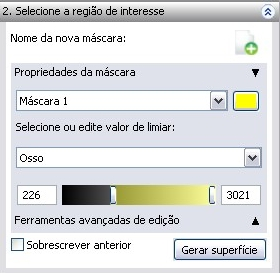
\includegraphics[scale=0.4]{ScreenHunter01Jan201144.jpg}
\caption{Seleção de região de interesse}
\label{fig:region_selection}
\end{figure}

Antes de iniciar a segmentação, é necessário configurar uma máscara. A máscara é uma
imagem com a região selecionada colorida e sobreposta à imagem original. Veja a figura
(\ref{fig:region_selection_masc})

\begin{figure}[!htb]
\centering
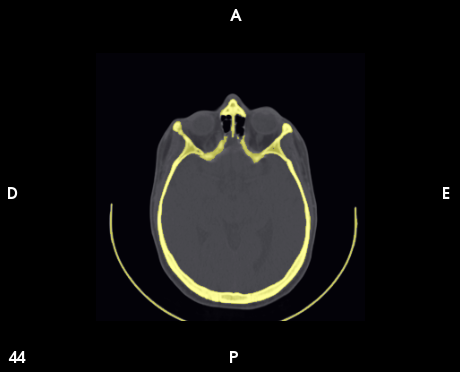
\includegraphics[scale=0.4]{limiar_principal}
\caption{Máscara (regiões em amarelo)}
\label{fig:region_selection_masc}
\end{figure}

Para alterar o limiar, pode-se utilizar a barra que representa os níveis de cinza na imagem (figura
\ref{fig:region_selection_bar}). É possível alterar o limiar inicial usando o controle deslizante
\textit{esquerdo} da barra. De forma semelhante, o limiar final pode ser alterado por meio do controle
\textit{direito}. É possível, ainda, digitar diretamente os valores desejados nas respectivas caixas
de texto nas extremidades da barra. Com a alteração dos valores, automaticamente a máscara será atualizada,
pintando somente os \textit{pixels} com intensidade dentro da faixa determinada.

\begin{figure}[!htb]
\centering
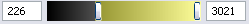
\includegraphics[scale=0.7]{limiar_barra}
\caption{Seleção dos \textit{pixels} com intensidade entre 226 e 3021 (Osso)}
\label{fig:region_selection_bar}
\end{figure}

Também existem valores pré-definidos de limiar de acordo com alguns tipos de tecido, como mostra a
figura \ref{fig:limiar_presets}. Basta selecionar o tecido desejado e a máscara será atualizada
automaticamente.

\begin{figure}[!htb]
\centering

\includegraphics[scale=0.6]{limiar_presets}
\caption{Caixa de seleção de valores pré-definidos de limiar}
\label{fig:limiar_presets}
\end{figure}

A tabela \ref{tab:limiar} mostra a faixa de níveis de cinza de acordo com o tipo de tecido ou material.

\begin{table}[h]
\centering
\caption{Limiares pré-definidos para alguns materiais}
\begin{tabular}{lcc}\\
\hline % este comando coloca uma linha na tabela
Material & Limiar inicial & Limiar final\\
\hline
\hline
Esmalte (Adulto) & 1553 & 2850\\
Esmalte (Criança) & 2042 & 3021\\
Osso & 226 & 3021\\
Osso Compacto (Adulto) & 662 & 1988\\
Osso Compacto (Criança) & 586 & 2198\\
Osso Esponjoso (Adulto) & 148 & 661\\
Osso Esponjoso (Criança) & 156 & 585\\
Personalizado & Def. Usuário & Def. Usuário\\
Tecido Epitelial (Adulto) & -718 & -177\\
Tecido Epitelial (Criança) & -766 & -202\\
Tecido Gorduroso (Adulto) & -205 & -51\\
Tecido Gorduroso (Criança) & -212 & -72\\
Tecido Muscular (Adulto) & -5 & 135\\
Tecido Muscular (Criança) & -25 & 139\\
Tecidos Moles & -700 & 225\\
\hline
\end{tabular}
\label{tab:limiar}
\end{table} 
\newpage

A tabela \ref{tab:limiar} é mais indicada para tomógrafos médicos. Nos tomógrafos odontológicos,
comumente as faixas de níveis de cinza são maiores e não regulares. Assim, é necessário utilizar
a barra de limiar (figura \ref{fig:region_selection_bar}) para ajustá-las.

Caso se deseje criar uma nova máscara, basta clicar no ícone do atalho presente no painel, dentro
do item \textbf{2. Selecione a região de interesse}. Veja a figura \ref{fig:shortcut_new_mask}.

\begin{figure}[!htb]
\centering

\includegraphics[scale=0.2]{object_add_original}
\caption{Atalho para criar nova máscara}
\label{fig:shortcut_new_mask}
\end{figure}

Clicando-se nesse atalho, uma nova janela será apresentada (figura \ref{fig:create_new_mask}).
Selecione a faixa de limiar desejada e clique em \textbf{OK}.

\begin{figure}[!htb]
\centering
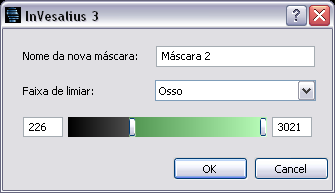
\includegraphics[scale=0.5]{limiar_janela}
\caption{Criar uma nova máscara}
\label{fig:create_new_mask}
\end{figure}

\newpage

Com uma máscara de segmentação configurada, é possível gerar a superfície 3D correspondente
às imagens em estudo. A superfície será composta por uma malha de triângulos. O próximo capítulo
trará maiores detalhes sobre esse tipo de superfície.

Para iniciar a geração, clique no botão \textbf{Gerar superfície} (figura \ref{fig:generate_surface}).
Caso já exista uma superfície gerada previamente, pode-se substituí-la pela nova. Para isso, basta
selecionar, \textbf{antes} da geração, a opção \textbf{Sobrescrever anterior}.

\begin{figure}[!htb]
\centering
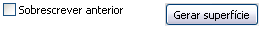
\includegraphics[scale=0.5]{generate_surface}
\caption{Botão Gerar superfície}
\label{fig:generate_surface}
\end{figure}

Após alguns instantes, a superfície será exibida na janela de visualização 3D do InVesalius
(figura \ref{fig:surface}).

\begin{figure}[!htb]
\centering
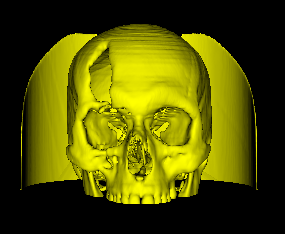
\includegraphics[scale=0.5]{3d_model}
\caption{Superfície 3D}
\label{fig:surface}
\end{figure}
 


\section{Segmentação manual (Edição de imagens)}

Há situações em que a segmentação por limiar não é eficiente, pois ela é aplicada ao conjunto
todo das imagens. Para aplicar a segmentação a imagens isoladas, pode-se usar a segmentação
manual. Com ela, é possível adicionar ou apagar uma determinada região da imagem que foi
segmentada por limiar. No entanto, a segmentação manual requer maior conhecimento de anatomia
por parte do usuário. Para utilizá-la, é necessário clicar em \textbf{Ferramentas avançadas
de edição} (figura \ref{fig:advanced_edition}) para abrir o painel de edição.

\begin{figure}[!htb]
\centering

\includegraphics[scale=0.6]{edicao_avancada}
\caption{Ferramentas avançadas de edição}
\label{fig:advanced_edition}
\end{figure}

O painel de edição aparece como mostra a figura \ref{fig:edition_slices_ref}.

\begin{figure}[!htb]
\centering
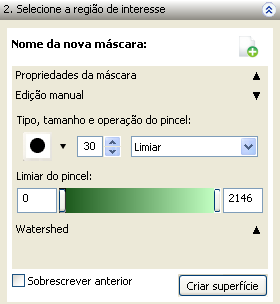
\includegraphics[scale=0.5]{edition_slices}
\caption{Painel de edição}
\label{fig:edition_slices_ref}
\end{figure}

Há dois tipos de pincel disponíveis para desenho: um em forma de círculo e outro em forma
de quadrado. Para escolher um pincel, clique no triângulo da lista de seleção para abri-la
e, a seguir, clique sobre o tipo escolhido. O pincel selecionado aparece no painel como
mostra a figura \ref{fig:brush_type}.

\begin{figure}[!htb]
\centering
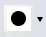
\includegraphics[scale=0.5]{edit_pencil}
\caption{Tipo de pincel}
\label{fig:brush_type}
\end{figure}

\newpage

Também é possível alterar o diâmetro do pincel, conforme mostra a figura \ref{fig:select_diameter}.

\begin{figure}[!htb]
\centering
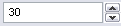
\includegraphics[scale=0.5]{diametro_pincel}
\caption{Seleção do diâmetro do pincel}
\label{fig:select_diameter}
\end{figure}

É necessário selecionar o tipo de operação que será realizada pelo pincel. As opções são as
seguintes:\\
\\
\textbf{Desenhar}, para pintar uma região que não foi selecionada;\\
\textbf{Apagar}, para remover uma região que foi selecionada;\\
\textbf{Limiar}, para remover uma região que está fora do limiar e foi selecionada, ou pintar
uma região que está dentro do limiar e não foi selecionada.\\

A figura \ref{fig:select_brush_operations} ilustra a lista de operações do pincel:

\begin{figure}[!htb]
\centering
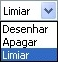
\includegraphics[scale=0.6]{select_brush_operation}
\caption{Seleção do tipo de operação do pincel}
\label{fig:select_brush_operations}
\end{figure}

A figura \ref{fig:noise_amalgaman} mostra um caso em que algumas imagens contêm ruídos
causados pela presença de prótese dentária de amálgama no paciente. Observe os "raios" 
saindo da região da arcada dentária. Isso ocorre porque a máscara de segmentação também
seleciona parte dos ruídos, pois eles estão na mesma intensidade do limiar para osso.

\begin{figure}[!htb]
\centering
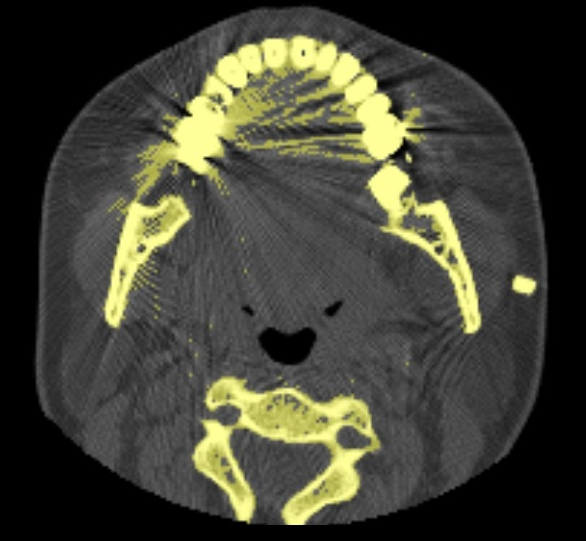
\includegraphics[scale=0.3]{noise_amalgam}
\caption{Imagem com ruído segmentada com limiar}
\label{fig:noise_amalgaman}
\end{figure}

A figura \ref{fig:surface_amagaman} ilustra como é uma superfície gerada a partir dessa
segmentação.

\begin{figure}[!htb]
\centering
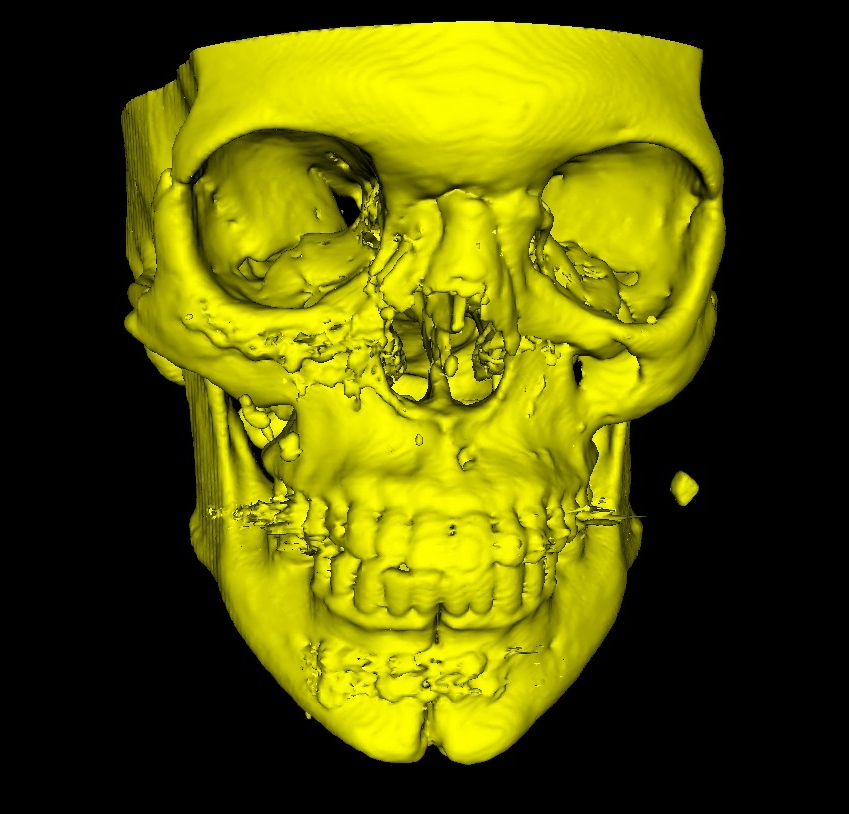
\includegraphics[scale=0.3]{case_almagam}
\caption{Superfície gerada a partir de imagem com ruído}
\label{fig:surface_amagaman}
\end{figure}

\begin{figure}[!htb]
\centering
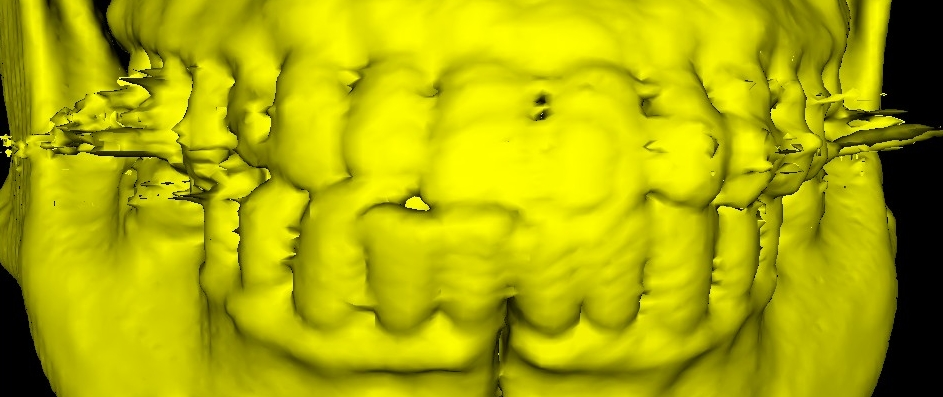
\includegraphics[scale=0.3]{case_almagam_zoom}
\caption{Zoom da região com ruído}
\label{fig:surface_amagaman_zoom}
\end{figure}

\newpage

Em casos como este, utilizando o editor, com o pincel na opção \textbf{Apagar}, mantenha o
botão \textbf{esquerdo} do mouse pressionado enquanto o \textbf{arrasta} sobre a região que
deseja remover (na máscara).

A figura \ref{fig:editor_amalgaman} mostra a imagem da figura \ref{fig:noise_amalgaman} após
edição.

\begin{figure}[!htb]
\centering
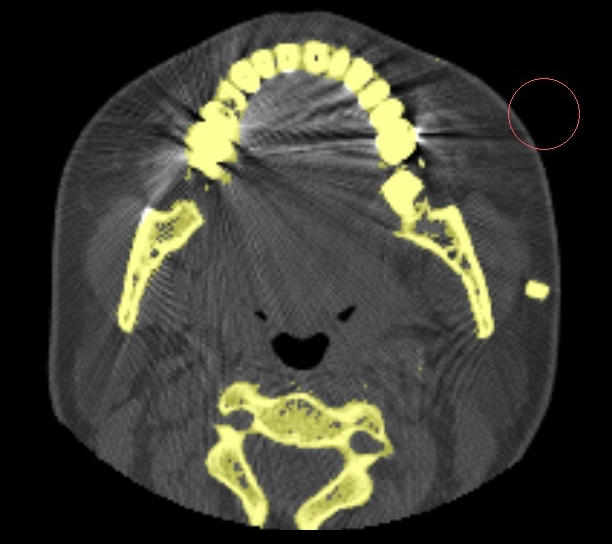
\includegraphics[scale=0.3]{editor_amagam}
\caption{Imagem com ruído removido}
\label{fig:editor_amalgaman}
\end{figure}

\begin{figure}[!htb]
\centering
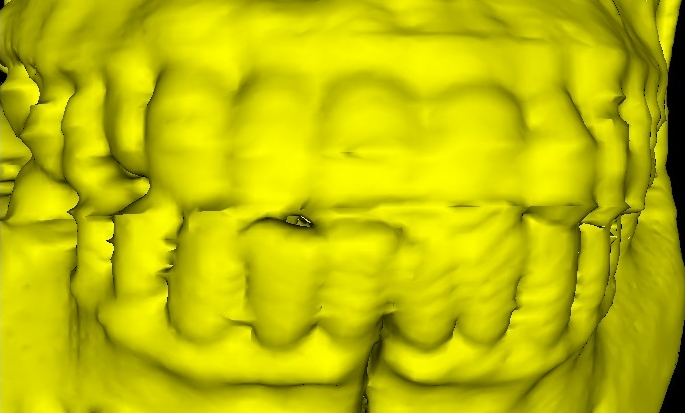
\includegraphics[scale=0.3]{edited_amalgam}
\caption{Superfície criada a partir da imagem com ruído removido}
\label{fig:surface_edited_amalgaman}
\end{figure}

\newpage
Realizada a edição, basta gerar a superfície a partir da imagem editada (figura
\ref{fig:surface_edited_amalgaman}). Como houve edição, ao clicar em \textbf{Criar superfície}, será
requerido se deseja gerar a superfície a partir do método \textbf{binário} ou utilizando o método de suavização
\textbf{Context aware smoothing} (figura \ref{fig:new_surface_edited}) para minimizar os "degraus" na superfície.
Demais detalhes serão discutidos no capítulo \ref{cap_surface}.
%\ref{fig:generate_surface}).

\begin{figure}[!htb]
\centering
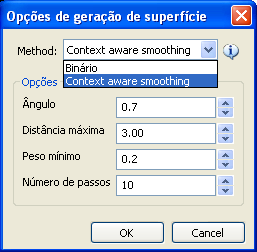
\includegraphics[scale=0.5]{create_surface_edited.png}
\caption{Método de criação de superfície}
\label{fig:new_surface_edited}
\end{figure}